\subsubsection{Vision Transformer Architecture}

\noindent The Vision Transformer (ViT) architecture comprises the following components:
\\

\noindent \textbf{Patch Embedding:} The process begins by dividing the input image into non-overlapping patches. Each patch is then transformed into an embedding through a linear projection. These embeddings are further enhanced with positional encodings. Positional encodings are crucial because transformers don't inherently understand the spatial relationships between elements, and these encodings provide information about the patch's position in the image.
\\
\begin{figure}[h]
    \centering
    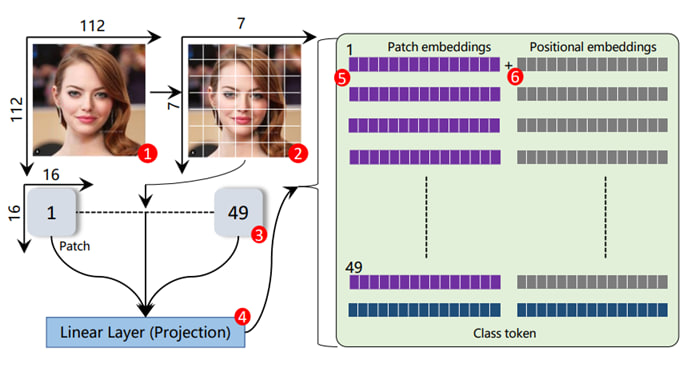
\includegraphics[width=6in]{img/patchembedding.jpg}
    \caption{Patch Embedding}
\end{figure}

\noindent \textbf{Transformer Encoder:} The patch embeddings are then processed through a stack of transformer encoder layers. Each of these layers consists of two main components: multi-head self-attention and feedforward neural networks.

\begin{enumerate}
    \item \textbf{Multi-head self-attention:} This mechanism allows the model to consider relationships between different patches, both locally and globally. It assigns different attention weights to different patches based on their relevance to each other. This is particularly powerful as it enables the model to capture long-range dependencies and relationships within the image.

    \item \textbf{Feedforward neural networks}: After the attention mechanism, the data passes through feedforward neural networks, which are designed to process and transform the information further. This step helps the model learn intricate features and patterns in the image data.
\end{enumerate}

\begin{figure}[h]
    \centering
    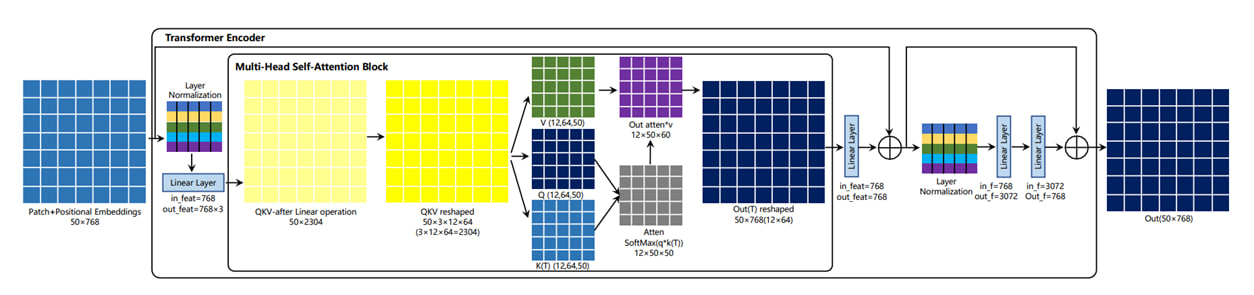
\includegraphics[width=6in]{img/encoderdetails.jpg}
    \caption{Transformer encoder}
\end{figure}
\noindent \textbf{Classification Head:} At the top of the architecture, there's a classification head. This final layer takes the transformed embeddings and uses them to predict whether an image is real or manipulated. It essentially makes the decision based on the features and patterns the model has learned throughout the previous layers.
\\

\begin{figure}[h]
    \centering
    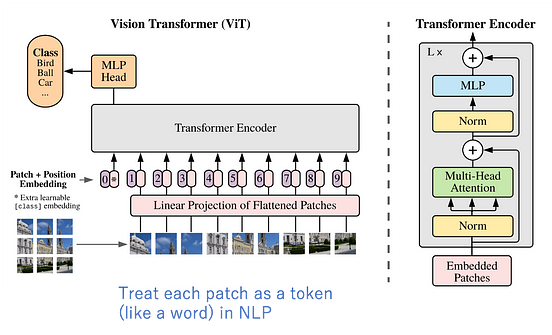
\includegraphics[width=6in]{img/visiontransformer.png}
    \caption{Vision Transformer Architecture}
\end{figure}

\newpage






